\chapter{Introduction}
\vspace{1cm}
\hfill%
\begin{minipage}{.4\linewidth}
    %\[ \argmax_{y \in \mathcal{Y}} f(x, y) \]
    %\dots I wish I could let it stand on its own like this, but of course there is more to come.
    %\flushright
    %\emph{Martial Hebert}
%Remember that all models are wrong;\\
%the practical question is how wrong do they have to be to not be useful.
Essentially, all models are wrong, but some are useful. 
\flushright%
\emph{George E. P. Box}

%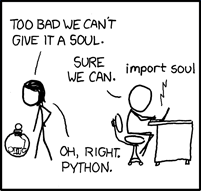
\includegraphics[width=\linewidth]{python_soul}%
%\flushright%
%Randall Munroe, \emph{xkcd.com}
\end{minipage}%
\\[2cm]
In computer vision research, the goal is to automatically extract information from an image.
In particular discerning semantic information, that is interpreting an image, is a prominent
research topic.
While much progress has been made in recent years, computer vision systems still lag behind
humans in most tasks that require semantic information. Often these tasks can be formulated
in terms of \emph{semantic classes}, meaning categories of parts, objects or scenes.
Examples include answering questions such as ``Is this a picture of a beach?'', ``How many
cars are there in this image?'' or even ``What objects lie on the table?''.
These questions illustrate a range of possible tasks involving semantic categories,
from classifying images of single objects, over localization and counting of object classes,
to parsing a scene fully into objects and object classes, together with their relations.
%
While humans can distinguish tens of thousands of object classes, and have
little trouble in interpreting complex scenes, current methods are often
restricted to a much smaller number of classes, and only have limited
capabilities to model interactions or relations.  We believe that
\emph{context} is one of the most important cues when it comes to classifying
objects, and therefore understanding scenes. Consequently, we target dense
labeling of scenes, taking object relations into account.  The task of densely
labeling image pixels into classes is called object class segmentation or
semantic segmentation.
\pagebreak

We choose this task in particular for several reasons:
\begin{itemize*}
    \item Pixel-level annotation provides highly detailed information about the scene.
    \item Joint estimation of multiple classes allows for the use of context.
    \item In contrast to category-agnostic segmentation approaches, object class segmentation
        has an unambiguous true labeling.
    \item A variety of manually annotated datasets is publicly available.
\end{itemize*}
%
Applications of semantic segmentation and scene understanding include automatic
image interpretation for retrieval, autonomous driving and mobile robotics.
While these are already important applications, we expect that with the
abundance of camera data, and the proliferation of mobile computing, even
more applications will emerge soon.

In the following we distinguish between the task of semantic segmentation,
which is usually distinguishing unstructured ``stuff'' classes such as road and
grass, and object class segmentation, which denotes the segmentation of very
structured classes, such as cars, planes and people. We consider four
different datasets in this thesis: the object class segmentation datasets
Graz02 and Pascal VOC 2010, and the semantic segmentation datasets MSRC-21, and
NYU V2.
%
Both tasks have the same ultimate goal of parsing, and therefore understanding,
images in terms of semantic classes, but usually employ  different mechanisms
to represent and process.

One of the bottlenecks in learning object class segmentation and semantic
segmentation is the availability of training data.  While unlabeled image data,
and even data with semantic
``tags'' is available in practically unlimited quantities, semantic annotation
on pixel level is only available through laborious manual annotation. 
Chapter~\ref{ch:semi_supervised} introduces an approach to cope with this
shortcoming of object class segmentation approaches by introducing a method to
find segmentations automatically from image level annotations.

The main part of this thesis investigates the use of structured learning~\citep{taskar2003max, tsochantaridis2006large}
algorithms to the task of semantic image segmentation. Both topics have received
much attention in the computer vision and machine learning communities
lately~\citep{ladicky2009associative, krahenbuhl2012efficient,
branson2013efficient, blake2011markov}.
Unfortunately, learning structured prediction in computer vision applications
is still little understood.
We focus on the use of conditional random fields~(CRFs), which have shown great
promise for computer vision applications. Using the paradigm of structural
support vector machines, it is possible to learn conditional random fields to
directly minimize a loss of interest. In particular, conditional random fields
allow to combine different cues, possibly produced by other approaches, in a
principled manner. One of the main difficulties with CRF approaches to computer
vision problems is that context in images is usually represented as a
neighborhood graph.  These graphs, by nature, contain many cycles, making
inference intractable in general. Consequently, learning algorithms have to
rely on approximate inference, with often unknown consequences to learning.

There have been several previous studies on learning structural support vector
machines, and learning for conditional random fields. The impact of approximate
inference was first investigated by \citet{finley2008training}, applying
structural support vector machines to multi-label data. Later, different works
investigated how to combine approximate inference and learning in a single
framework. \citet{meshi2010learning, komodakis2011efficient}, and
\citet{hazan2010primal} approached the problem using duality, and formulate
learning and inference as a joint optimization problem.
\citet{stoyanov2011empirical}, and later \citet{jancsarylearning} and
\citet{krahenbuhlparameter} formulate learning structured prediction as
optimizing a \emph{prediction engine}, that takes into account all aspects of
the model, in particular the inference algorithm used.
In this work, on the other hand, we follow the well-established algorithms for
learning structural support vector machines, and investigate how we can use the
available inference algorithms to obtain good results within a reasonable
time-frame.

\citet{nowozin2010parameter} provide a detailed evaluation of different aspects
of learning object class segmentation, that is somewhat orthogonal to this
work. Their work considers the choice of features, number of superpixels and
pairwise potentials for conditional maximum likelihood learning of
tree-structured CRFs.  \citet{nowozin2010parameter} also compare conditional
maximum likelihood learning with maximum margin learning, finding little
difference in accuracy.
We focus our work on the more popular neighborhood graphs, which do not allow
for efficient inference.  Therefore, conditional maximum likelihood learning is
intractable in our setting. For our studies, we fix the considered feature set,
and vary the maximum margin learning algorithm. Despite this seemingly limited
setup, we can make out large differences in the applicability of some of the
commonly used methods. For comparison, we also evaluate the learning algorithms
on chain CRFs, where efficient inference is possible.
More recently, \citet{lucchi2013learning} proposed a novel algorithm for
efficiently learning structured prediction for semantic segmentation, using
approximate inference. In Chapter~\ref{ch:exact_learning}, we introduce an
algorithm that runs in similar time to the one proposed by
\citet{lucchi2013learning}, but is able to learn a CRF to the exact optimum on
the same dataset.


\section{List of Contributions}
This thesis contains the following contributions:
\begin{itemize}
\item Introducing a clustering algorithm that improves upon widely used
    approaches from the literature.
\item Demonstrating a scalable algorithm for weakly supervised object class segmentation.
\item Providing a general and efficient open source software framework for structured prediction.
\item Analysing max-margin learning algorithms with exact or approximate inference in different applications.
\item Showing that exact learning for semantic segmentation and object class
    segmentation is possible in practice, even in loopy graphs.
\end{itemize}

\section{Thesis Outline}
Before we delve into semantic segmentation and object class recognition, we
first investigate a general clustering algorithm in Chapter~\ref{ch:itm}.
Clustering is an important step in most semantic segmentation pipelines, in at
least two places: bottom-up segmentation and creation of dictionaries for
feature learning. We introduce a novel information theoretic algorithm that
compares favourably with algorithms from the literature.  While we do not apply
our algorithm to the task of bottom-up segmentation, this is a promising avenue
for future research.

We introduce an algorithm for semi-supervised learning of object class
segmentation in Chapter~\ref{ch:semi_supervised}, motivated by the problem of
annotating training data for semantic segmentation.

The central topic of this thesis is introduced in
Chapter~\ref{ch:structured_pystruct}, which also introduces our software
library for implementing structured learning and prediction algorithms.

Chapter~\ref{ch:comparison} gives a quantitative comparison of the most widely
used structured prediction algorithms in diverse settings.
%, focusing on which algorithm is best to %TODO formulation
%use in a given situation.
In particular, we investigate learning behavior for
semantic segmentation on several datasets.

The problem of learning with approximate inference is investigated in
Chapter~\ref{ch:exact_learning}.  We develop a strategy for efficient caching
and a combination of inference algorithms that allows us to learn SSVMs for
semantic image segmentation exactly, even though the involved factor graphs
contain many loops. We demonstrate our algorithm on the Pascal VOC 2010 and MSRC-21 datasets,
and provide state-of-the-art results on the MSRC-21 dataset.

Finally, Chapter~\ref{ch:nyu} applies the methods developed in
Chapter~\ref{ch:structured_pystruct} and Chapter~\ref{ch:exact_learning} to the
problem of semantic annotation with structure classes in RGB-D data. We
demonstrate that we are able to learn meaningful spacial relations, and improve
upon the state-of-the-art on the NYU V2 datasets.

\section{Publications}
The main material of this thesis has either been published in conference
proceedings or has been submitted to conferences or journals. We now list the
relevant publications.
\begin{description}
    \item[Chapter~\ref{ch:itm}] \emph{Information Theoretic Clustering using
        Minimum Spanning Trees} Andreas C. M\"uller, Sebastian Nowozin and
        Christoph H. Lampert. Published in the proceedings of the German
        Conference on Pattern Recognition.
    \item[Chapter~\ref{ch:semi_supervised}] \emph{Multi-Instance Methods for
        Partially Supervised Image Segmentation} Andreas C. M\"uller and Sven
        Behnke. Published in the proceedings of the IARP Worshop on Partially
        Supervised Learning.
    \item[Chapter~\ref{ch:structured_pystruct}] \emph{PyStruct - Structured
        Prediction in Python} Andreas C. M\"uller and Sven Behnke. Submitted to
        the Journal of Machine Learning Research, Open Source Software track.
    \item[Chapter~\ref{ch:exact_learning}] \emph{Learning a Loopy Model for
        Semantic Segmentation Exactly}. Andreas C. M\"uller and Sven Behnke.
        Submitted to the International Conference on Computer Vision Theory and
        Applications.
    \item[Chapter~\ref{ch:nyu}] \emph{Learning Depth-Sensitive Conditional
        Random Fields for Semantic Segmentation}. Andreas C. M\"uller and Sven
        Behnke. Submitted to the International Conference on Robotics and
        Automation.
\end{description}
